\documentclass[11pt]{amsart}
\usepackage[margin=1.1in]{geometry}
\usepackage{amssymb,mathtools}
\usepackage{graphicx}
\usepackage{booktabs}
\usepackage{tikz}
\usetikzlibrary{arrows.meta,positioning}
\usepackage{xurl}
\usepackage[colorlinks=false,hidelinks]{hyperref}
\graphicspath{{./}{figures/}}
\numberwithin{equation}{section}
\theoremstyle{plain}
\newtheorem{thm}{Theorem}[section]
\newtheorem{lem}[thm]{Lemma}
\newtheorem{prop}[thm]{Proposition}
\newtheorem{cor}[thm]{Corollary}
\theoremstyle{remark}
\newtheorem{rem}[thm]{Remark}
\newcommand{\Z}{\mathbb{Z}}
\newcommand{\Q}{\mathbb{Q}}
\newcommand{\C}{\mathbb{C}}
\newcommand{\cO}{\mathcal{O}}
\newcommand{\cA}{\mathcal{A}}
\newcommand{\cE}{\mathcal{E}}
\newcommand{\e}{\mathbf{e}}
\newcommand{\pmi}{\phi_{-2,1}}
\newcommand{\pz}{\phi_{0,1}}
\newcommand{\tPhi}{\widetilde{\Phi}}


\title{Positive First-Row Black Hole Indices in CHL Models}
\author{Deep Bhattacharjee}
\address{Formerly, Electro-Gravitational Space Propulsion Laboratory (EGSPL), Bhubaneswar, Odisha 751030, India; formerly, University of Calcutta (Heramba Chandra College), 23/49 Gariahat Road, Golpark, Kolkata 700029, West Bengal, India}
\email{d.bhattacharjee@erl-forschung.de}
\subjclass[2020]{11F50 (primary); 11F37, 11F27, 81T30, 83E30}
\keywords{CHL models, single-centred black holes, quaternion orders}

\begin{document}
\begin{abstract}
In the $\Z_3$, $\Z_5$ and $\Z_7$ CHL models, every single-centred black hole with electric charge $Q^2=2/N$ has a positive index, as Sen predicted. The proof writes the relevant mock Jacobi form in closed form through an eta quotient, the theta series of a maximal quaternion order and Hurwitz class numbers.
\end{abstract}
\maketitle


%%==================================================================
\section{Introduction}
%%==================================================================

A quarter-BPS dyon in an $\mathcal N=4$ string theory in four dimensions carries an electric charge $Q$ and a magnetic charge $P$, and its protected index is the helicity trace $B_6$. When the charges admit a single-centred black hole, the horizon is spherically symmetric, its microstates carry zero angular momentum, and the twelve fermion zero modes of the broken supersymmetries fix the overall sign: the black hole contributes $-B_6>0$. Sen turned this observation into a prediction about Fourier coefficients of Siegel modular forms \cite{Sen11}: the index $d_*(Q,P)$ of the single-centred black hole, extracted from the inverse of the dyon partition function along the attractor contour, is positive.\footnote{The argument is physical. The single-centred black hole preserves an $SU(2)$ rotation symmetry, so its states have $J_3=0$ after the fermion zero modes are removed, and then $(-1)^{2J_3}=1$ for every state. Sen checked the sign on the charges of his Tables~1--5, for heterotic string theory on $T^6$ and for the CHL models of orders $2,3,5,7$ \cite{Sen11}; the entropy function and attractor background behind the statement are reviewed in \cite{Sen08}.}

For type~II string theory on $K3\times T^2$, where the partition function is the inverse of the Igusa cusp form $\Phi_{10}$ \cite{DVV97}, the prediction is now a theorem. Bringmann and Murthy proved it for the two smallest magnetic charges by writing the relevant mock modular forms through class numbers \cite{BM13}, and Rossell\'o treated all charges through a mixed Rademacher series \cite{Ros24}. The CHL models \cite{CHL95} are $\Z_N$ orbifolds in which the $\Z_N$ acts on $K3$ by a symplectic automorphism and on $T^2$ by a shift; their partition functions $\tPhi_k$ are Siegel modular forms of weight $k$ for congruence subgroups of $Sp(2,\Z)$ \cite{JS06,DJS06}. Bhand, Sen and Singh proved that the Fourier--Jacobi coefficients of $1/\tPhi_k$ are meromorphic Jacobi forms whose finite parts are mock Jacobi forms, and that on an explicit set of charges the single-centred index is a Fourier coefficient of such a finite part \cite{BSS25}. For $N=2$ the conjecture has been proved for every charge in \cite{Bha26a}, and the companion paper \cite{Bha26b} settles the toroidal compactifications and the heterotic string under stated arithmetic conditions.

This paper treats the CHL models of prime order $N=3,5,7$, for which $k+2=24/(N+1)$, so $k=4,2,1$. The charges are normalised so that
\begin{equation}\label{eq:charges}
m=\tfrac{N}{2}Q^2,\qquad n=\tfrac12P^2,\qquad \ell=Q\cdot P
\end{equation}
are integers, and the discriminant is $D=Q^2P^2-(Q\cdot P)^2=4mn/N-\ell^2$. The first row is $m=1$, that is $Q^2=2/N$, the smallest electric charge of the model.

\begin{thm}\label{thm:main}
Let $N\in\{3,5,7\}$. In the $\Z_N$ CHL model, $d_*(Q,P)>0$ for every pair of charges with $Q^2=2/N$ and $D>0$.
\end{thm}

The proof rests on a closed formula. Write $\e(t)=e^{2\pi i t}$, $x=\e(\sigma/N)$, $y=\e(v)$, let $\pmi$ and $\pz$ be the weak Jacobi forms of weight $-2$ and $0$ and index one \cite[\S9]{EZ85}, let $H(\sigma,v)=\sum H(4a-r^2)\e(a\sigma+rv)$ be the generating function of the Hurwitz class numbers, and let $g(\tau)=\eta(\tau)^{k+2}\eta(N\tau)^{k+2}$. Let $\cO_N$ be a maximal order in the quaternion algebra over $\Q$ ramified exactly at $N$ and $\infty$, and let $w$ be an element of its dual lattice with reduced norm $1/N$ (Section~\ref{sec:theta}).

\begin{thm}\label{thm:closed}
Let $N\in\{3,5,7\}$ and let $\varphi^F_1$ be the finite part of the first Fourier--Jacobi coefficient of $1/\tPhi_k$. Then
\begin{equation}\label{eq:closed}
g\!\left(\tfrac{\sigma}{N}\right)\varphi^F_1(\sigma,v)=W_N\!\left(\tfrac{\sigma}{N}\right)\pmi(\sigma,v)-\frac{\hat f_N}{6}\,\Theta_N(\sigma,v)-2\hat f_N\,H(\sigma,v),
\end{equation}
where $\Theta_N(\sigma,v)=\sum_{\xi\in\cO_N}x^{\operatorname{nrd}\xi}\,y^{\operatorname{trd}(\xi\bar w)}$, the constants are $\hat f_3=27$, $\hat f_5=14$, $\hat f_7=9$, and
\begin{equation}\label{eq:WN}
W_3=\tfrac{3}{80}\bigl(E_4(\tau)-E_4(3\tau)\bigr),\quad
W_5=15\,\frac{\eta(5\tau)^{10}}{\eta(\tau)^2},\quad
W_7=3\,\theta_{[1,1,2]}(\tau)\,\frac{\eta(7\tau)^7}{\eta(\tau)},
\end{equation}
with $\theta_{[1,1,2]}(\tau)=\sum_{a,b\in\Z}q^{a^2+ab+2b^2}$.
\end{thm}

The number $\hat f_N$ is the coefficient of $q$ in $1/g(\tau)$, so it is the residue that defines the polar part, and the factor $-2\hat f_N$ in front of $H$ is the one forced by the shadow. Formula \eqref{eq:closed} is the analogue at levels $3,5,7$ of the identity found for $N=2$ in \cite{Bha26a}, where the theta series of $D_4$ appears; $D_4$ is the Hurwitz order, the maximal order ramified at $2$ and $\infty$, so the quaternion orders of discriminant $N$ unify the four cases.

The sign follows from \eqref{eq:closed} in two steps. After the twist $y\mapsto -y$ that turns $(-1)^{\ell+1}$ into a common sign, the first term has nonnegative coefficients, the second and third terms can be negative only when $\ell$ is odd, and the first term outgrows them: it is a cusp form of weight four times a function with a fixed sign pattern, while the theta series and the class numbers grow at most linearly. The finitely many small cases are read off exactly. Dividing by $g$, whose inverse has positive coefficients, then preserves positivity. Figure~\ref{fig:map} shows the structure.

\begin{figure}[t]
\centering
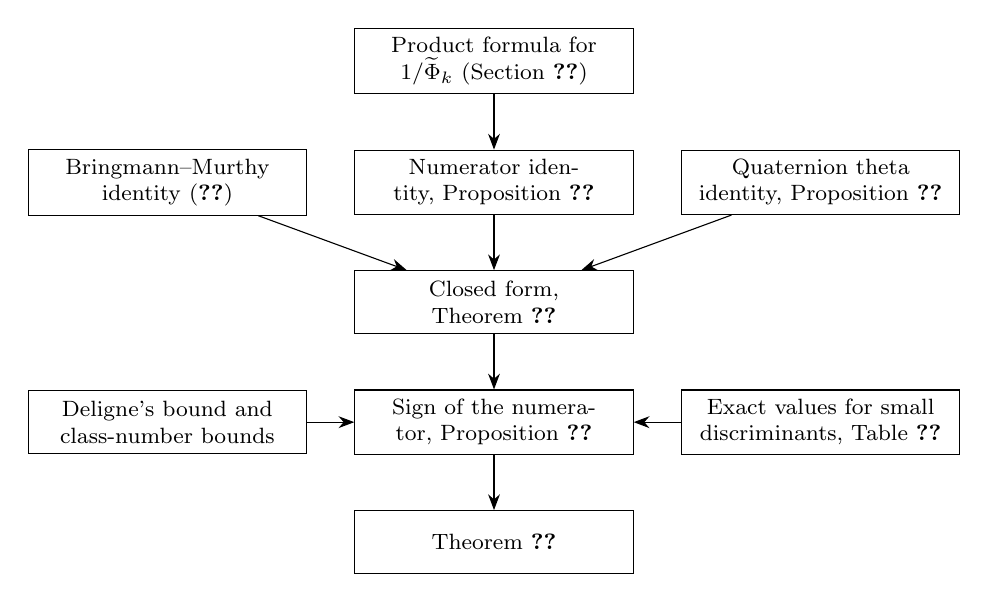
\begin{tikzpicture}[node distance=7mm and 6mm, every node/.style={draw, rectangle, align=center, font=\footnotesize, minimum height=8mm, text width=33mm}, >={Stealth[length=2mm]}]
\node (prod) {Product formula for $1/\tPhi_k$ (Section~\ref{sec:pf})};
\node (num) [below=of prod] {Numerator identity, Proposition~\ref{prop:num}};
\node (bm) [left=of num] {Bringmann--Murthy identity \eqref{eq:BM}};
\node (th) [right=of num] {Quaternion theta identity, Proposition~\ref{prop:theta}};
\node (cl) [below=of num] {Closed form, Theorem~\ref{thm:closed}};
\node (sg) [below=of cl] {Sign of the numerator, Proposition~\ref{prop:sign}};
\node (ex) [right=of sg] {Exact values for small discriminants, Table~\ref{tab:small}};
\node (an) [left=of sg] {Deligne's bound and class-number bounds};
\node (mt) [below=of sg] {Theorem~\ref{thm:main}};
\draw[->] (prod) -- (num); \draw[->] (num) -- (cl); \draw[->] (bm) -- (cl); \draw[->] (th) -- (cl);
\draw[->] (cl) -- (sg); \draw[->] (an) -- (sg); \draw[->] (ex) -- (sg); \draw[->] (sg) -- (mt);
\end{tikzpicture}
\caption{The structure of the proof. Each arrow is an implication proved in the section named in the box it leaves.}
\label{fig:map}
\end{figure}

Section~\ref{sec:pf} recalls the partition function, the decomposition of Bhand, Sen and Singh and the region in which the finite part computes $d_*$. Section~\ref{sec:num} proves the numerator identity, Section~\ref{sec:theta} the theta identity, and Section~\ref{sec:closed} assembles Theorem~\ref{thm:closed}. Section~\ref{sec:sign} proves Theorem~\ref{thm:main}. Section~\ref{sec:checks} compares the formulas with the product formula and with Sen's tables and records an exact check of all charges with $Q^2\le 12/N$ in a large box. Section~\ref{sec:all} describes what an extension to all charges requires.

%%==================================================================
\section{The Partition Function and the Single-Centred Index}\label{sec:pf}
%%==================================================================

\subsection{Twisted elliptic genera}
Let\[\pmi(\tau,z)=-\frac{\theta_1(\tau,z)^2}{\eta(\tau)^6},\qquad \pz(\tau,z)=4\sum_{j=2}^4\frac{\theta_j(\tau,z)^2}{\theta_j(\tau)^2},\]so that $\pmi=\zeta-2+\zeta^{-1}+O(q)$ and $\pz=\zeta+10+\zeta^{-1}+O(q)$ with $\zeta=\e(z)$. We write $\alpha(4a-r^2)$ for the coefficient of $q^a\zeta^r$ in $\pmi$. Let
\begin{equation}\label{eq:EN}
E_N(\tau)=\frac{NE_2(N\tau)-E_2(\tau)}{N-1}=1+\frac{24}{N-1}\sum_{n\ge1}\sigma^{(N)}(n)q^n,\qquad \sigma^{(N)}(n)=\sum_{d\mid n,\ N\nmid d}d,
\end{equation}
the weight-two Eisenstein series of $\Gamma_0(N)$; it spans $M_2(\Gamma_0(N))$ for $N\in\{2,3,5,7\}$, since these levels have genus zero.\footnote{The dimension of $S_2(\Gamma_0(N))$ equals the genus of the modular curve $X_0(N)$, which is zero for $N=2,3,5,7$. So for these levels every holomorphic modular form of weight two is a multiple of $E_N$, and identities of weight two reduce to a comparison of constant terms.}
The twisted elliptic genera of $K3$ for a symplectic automorphism of prime order $N$ are \cite{JS06,DJS06}
\begin{equation}\label{eq:genera}
\begin{aligned}
F^{(0,0)}&=\tfrac{2}{N}\pz,\qquad F^{(0,s)}=\tfrac{2}{N(N+1)}\pz+\tfrac{2}{N+1}\pmi\,E_N(\tau)\quad(1\le s\le N-1),\\
F^{(r,rt)}&=\tfrac{2}{N(N+1)}\pz-\tfrac{2}{N(N+1)}\pmi\,E_N\!\left(\tfrac{\tau+t}{N}\right)\quad(1\le r\le N-1,\ t\in\Z/N).
\end{aligned}
\end{equation}
Each $F^{(r,s)}$ is a weak Jacobi form of weight $0$ and index $1$ for $\Gamma(N)$, and $SL_2(\Z)$ permutes them by $F^{(r,s)}|\gamma=F^{(r,s)\gamma}$. For $N=2$ these are the functions used in \cite{Bha26a}. Write $F^{(r,s)}=\sum_{b\in\{0,1\}}\sum_{j\equiv b\,(2)}\sum_{n\in\Z/N}c_b^{(r,s)}(4n-j^2)q^n\zeta^j$.

\subsection{The product formula}
The dyon partition function is \cite{DJS06}
\begin{equation}\label{eq:product}
\tPhi_k(\rho,\sigma,v)=\e\!\left(\rho+\tfrac{\sigma}{N}+v\right)\prod_{b=0}^{1}\prod_{r=0}^{N-1}\prod_{\substack{\kappa'\in\Z+r/N,\ l\in\Z,\ j\in2\Z+b\\ \kappa',l\ge0,\ j<0\text{ if }\kappa'=l=0}}\bigl(1-\e(\kappa'\sigma+l\rho+jv)\bigr)^{E(N\kappa',l,j)},
\end{equation}
with $E(\kappa,l,j)=\sum_{s=0}^{N-1}\e(-sl/N)\,c_b^{(r,s)}(4\kappa l/N-j^2)$, $r\equiv\kappa$, and the index of $(Q,P)$ is $(-1)^{Q\cdot P+1}$ times the coefficient of $\e(m\rho)x^ny^\ell$ in $1/\tPhi_k$ on the attractor contour \cite{JS06,DJS06,Sen08}, in the notation \eqref{eq:charges}.

The exponents with $l=0$ are read off from the constant terms of \eqref{eq:genera}. For $|j|=1$ only $r=0$ contributes, with $\sum_s c^{(0,s)}(-1)=2$. For $j=0$ the exponent is $\sum_sc^{(0,s)}(0)=(44-4N)/(N+1)$ when $N\mid\kappa$ and $\sum_t c^{(r,rt)}(0)=24/(N+1)$ otherwise. Together with the prefactor they give the first Fourier--Jacobi coefficient
\begin{equation}\label{eq:phim1}
\varphi_{-1}(\sigma,v)=\frac{1}{g(\sigma/N)\,\pmi(\sigma,v)},
\end{equation}
because $\pmi=(\zeta-2+\zeta^{-1})\prod_n(1-q^n\zeta)^2(1-q^n\zeta^{-1})^2(1-q^n)^{-4}$ and $-2(k+2)+4=-(44-4N)/(N+1)$.\footnote{The check is the identity $48/(N+1)-4=(44-4N)/(N+1)$. The factors $(1-x^\kappa)$ with $N\nmid\kappa$ carry the exponent $24/(N+1)=k+2$ of $\eta(\sigma/N)^{k+2}$, and those with $N\mid\kappa$ carry the sum of the exponents of $\eta(\sigma/N)^{k+2}$ and $\eta(\sigma)^{k+2}$, minus the four powers of $1-p^n$ in $\pmi$, $p=x^N$.}

\subsection{The numerator}
Taking logarithms of the factors with $l\ge1$ and collecting powers of $\e(\rho)$ gives
\begin{equation}\label{eq:exp}
\frac{1}{\tPhi_k}=\varphi_{-1}\,\e(-\rho)\exp\Bigl(\sum_{L\ge1}L_L(\sigma,v)\,\e(L\rho)\Bigr),
\qquad L_L=\sum_{lt=L}\frac1t\sum_{\kappa\ge0}\sum_jE(\kappa,l,j)\,x^{\kappa t}y^{jt}.
\end{equation}

\begin{lem}\label{lem:hecke}
For every $L\ge1$,
\[
L_L(\sigma,v)=\sum_{lt=L}\frac{1}{lt}\sum_{r,s\in\Z/N}\ \sum_{u=0}^{l-1}\e\!\left(-\frac{ls+ur}{N}\right)F^{(r,s)}\!\left(\frac{t\sigma+u}{l},\,tv\right).
\]
Consequently $L_L$ is a weak Jacobi form of weight $0$ and index $L$ for $\Gamma(NL)$, acting on $\sigma$; it is even and holomorphic in $v$ and weak at every cusp.
\end{lem}

\begin{proof}
Put $F^{(r)}_l=\sum_s\e(-sl/N)F^{(r,s)}$. By \eqref{eq:genera} the coefficient of $q^n\zeta^j$ in $F^{(r)}_l$ vanishes unless $Nn\equiv rl\pmod N$: for $r=0$ the $q$-powers are integral, and for $r\ne0$ the sum over $s=rt$ multiplies the coefficient of $q^{c/N}$ in $\pmi E_N((\tau+t)/N)$ by $\sum_t\e(-rtl/N+tc/N)$, which is $N$ or $0$ according as $c\equiv rl$ or not. The coefficient of $q^n\zeta^j$ in $F^{(r)}_l$ is $E(\kappa,l,j)$ when $n=\kappa l/N$. For such $n$ the sum $\frac1l\sum_{u=0}^{l-1}\e(u(n/l-r/N))$ equals $1$ when $\kappa=Nn/l$ is an integer congruent to $r$ and $0$ otherwise, since $n/l-r/N\in\frac1l\Z$. Substituting $\tau=(t\sigma+u)/l$ turns $q^n$ into $x^{\kappa t}\e(un/l)$, and $z=tv$ turns $\zeta^j$ into $y^{jt}$; this proves the formula. For $\gamma=\left(\begin{smallmatrix}a&b\\c&e\end{smallmatrix}\right)\in\Gamma(NL)$ and $M=\left(\begin{smallmatrix}t&u\\0&l\end{smallmatrix}\right)$ one has
\[
M\gamma M^{-1}=\begin{pmatrix}a+uc/t& \bigl(tb+u(e-a)-u^2c/t\bigr)/l\\ lc/t& e-uc/t\end{pmatrix}\in\Gamma(N),
\]
because $c/t$, $b$ and $e-a$ are divisible by $Nl$; so every term is invariant. The elliptic property of index $L$ follows as in \cite[Lemma~1]{Bha26a}: the shift $v\mapsto v+\lambda\sigma+\mu$ moves $tv$ by $\lambda l\tau'+(t\mu-\lambda u)$ with $\tau'=(t\sigma+u)/l$, and the index-one law of $F^{(r,s)}$ produces $\e(-\lambda^2L\sigma-2\lambda Lv)$. For $\gamma\in SL_2(\Z)$ one has $M\gamma=\gamma'M'$ with $\gamma'\in SL_2(\Z)$ and $M'$ upper triangular of determinant $L$, and $SL_2(\Z)$ permutes the $F^{(r,s)}$, none of which has a negative power of $q$; so each term is weak at every cusp.
\end{proof}

Expanding \eqref{eq:exp} to first order beyond the leading term,
\begin{equation}\label{eq:numerator}
g\!\left(\tfrac\sigma N\right)\pmi(\sigma,v)\,\varphi_1(\sigma,v)=L_2+\tfrac12L_1^2=:\cE_N,
\end{equation}
a weak Jacobi form of weight $0$ and index $2$ for $\Gamma(2N)$ by Lemma~\ref{lem:hecke}.

\subsection{Polar part, finite part and the single-centred index}
By \cite[Theorem~5.2]{BSS25} each $\varphi_m$ is a meromorphic Jacobi form of weight $-k$ and index $m$ with double poles at $v\in\Z\sigma+\Z$, and its polar part is \cite[(5.45)]{BSS25}
\begin{equation}\label{eq:polar}
\varphi^P_m=\frac{\hat f(m)}{g(\sigma/N)}\cA_{2,m},\qquad \cA_{2,m}(\sigma,v)=\sum_{s\in\Z}\frac{p^{ms^2+s}y^{2ms+1}}{(1-p^sy)^2},\qquad p=\e(\sigma),
\end{equation}
where $\hat f(m)$ is the coefficient of $q^m$ in $1/g(\tau)$; thus $\hat f(1)=27,14,9$ for $N=3,5,7$. The finite part $\varphi^F_m=\varphi_m-\varphi^P_m=\sum c^F_m(n,\ell)x^ny^\ell$ is a mock Jacobi form. Let $\cA$ be the set of charges with $m,n>0$, $D>0$ and
\begin{equation}\label{eq:setA}
\min_{\substack{m_1\in N\Z,\ s\in\Z\\ m_1\mid s(s+1)}}\Bigl[(m_1\ell+2ms+m)^2+m_1^2D\Bigr]\ \ge\ m^2.
\end{equation}
By \cite[Theorem~5.4(a) and (5.57)]{BSS25}, for every charge in $\cA$,
\begin{equation}\label{eq:dstar}
d_*(Q,P)=(-1)^{\ell+1}c^F_m(n,\ell).
\end{equation}

\begin{lem}\label{lem:first}
Every charge with $m=1$ and $D>0$ lies in $\cA$. The coefficient $c^F_1(n,\ell)$ depends only on $\Delta=ND=4n-N\ell^2$, and $\Delta$ determines the parity of $\ell$.
\end{lem}

\begin{proof}
If $m_1=0$ then $s(s+1)=0$ and the bracket equals $(2s+1)^2=1$. If $m_1\ne0$ then $m_1^2\ge N^2$ and $D=\Delta/N\ge1/N$, so the bracket is at least $N\ge1$. The finite part is a mock Jacobi form of index one, hence has the elliptic property under $v\mapsto v+\lambda\sigma+\mu$, and its coefficients depend on $4n/N-\ell^2$ and $\ell\bmod2$ \cite[\S2]{EZ85}; since $N$ is odd, $\Delta\equiv\ell^2\cdot(-N)\pmod4$ fixes $\ell\bmod2$.
\end{proof}

%%==================================================================
\section{The Numerator Identity}\label{sec:num}
%%==================================================================

\begin{prop}\label{prop:num}
For $N=3,5,7$,
\begin{equation}\label{eq:num}
\cE_N=\alpha_N\,\pz^2-2\alpha_N\,E_N(\tfrac\sigma N)\,\pz\pmi+\gamma_N\,\pmi^2,\qquad \alpha_N=\frac{\hat f(1)}{144},
\end{equation}
where $\pz,\pmi$ are taken at $(\sigma,v)$ and
\begin{align*}
\gamma_3&=\tfrac{3}{160}E_4(\tfrac\sigma3)+\tfrac{27}{160}E_4(\sigma),\\
\gamma_5&=-\tfrac{1}{288}E_4(\tfrac\sigma5)-\tfrac{19}{288}E_4(\sigma)+\tfrac16E_5(\tfrac\sigma5)^2,\\
\gamma_7&=-\tfrac{1}{960}E_4(\tfrac\sigma7)-\tfrac{29}{960}E_4(\sigma)+\tfrac{3}{32}E_7(\tfrac\sigma7)^2.
\end{align*}
\end{prop}

\begin{proof}
Every term of \eqref{eq:num} is a weak Jacobi form of weight $0$ and index $2$ for $\Gamma(2N)$, even in $v$: the functions $E_4(\sigma/N)$, $E_4(\sigma)$ and $E_N(\sigma/N)$ are modular for the group $\{\left(\begin{smallmatrix}a&b\\c&d\end{smallmatrix}\right)\in SL_2(\Z):N\mid b\}$, which contains $\Gamma(N)$, and holomorphic at every cusp. Let $G$ be the difference of the two sides and expand $G=\chi_0(\sigma)+\chi_2(\sigma)v^2+\chi_4(\sigma)v^4+\cdots$. If $\chi_0=\dots=\chi_{\nu-2}=0$, the lowest order in $v$ of the transformation law shows that $\chi_\nu$ is a modular form of weight $\nu$ for $\Gamma(2N)$, holomorphic at the cusps because $G$ is weak \cite[\S3]{EZ85}. The index of $\overline{\Gamma(2N)}$ in $PSL_2(\Z)$ is $72$, $360$, $1008$ for $N=3,5,7$, and the width of the cusp $\infty$ is $2N$, so by Sturm's theorem \cite{Stu87} a form of weight $\nu\le4$ vanishes once its coefficients vanish through $x^{\nu\cdot\mathrm{index}/24}$, that is through $x^{12}$, $x^{60}$, $x^{168}$.\footnote{Sturm's bound for weight $k$ on a subgroup of index $\mu$ in $PSL_2(\Z)$ is $k\mu/12$ in the local parameter $\e(\sigma/w)$ at a cusp of width $w$. Here $w=2N$ and $x=\e(\sigma/N)$ is the square of the local parameter, which halves the bound.} We expanded both sides from \eqref{eq:exp}, \eqref{eq:genera} and \eqref{eq:product} in exact rational arithmetic through $x^{40}$, $x^{70}$ and $x^{175}$ respectively; they agree. Hence $\chi_0=\chi_2=\chi_4=0$. For each $\sigma$ the entire function $G(\sigma,\cdot)$ then vanishes to order at least six at $v=0$, while a nonzero function with the elliptic property of index two has exactly four zeros in a period parallelogram \cite[Theorem~1.2]{EZ85}. Hence $G=0$.
\end{proof}

The coefficient of $\pz^2$ is fixed by the polar part: the identity of Bringmann and Murthy \cite[Section~3]{BM13}
\begin{equation}\label{eq:BM}
\frac{\pz(\sigma,v)^2}{\pmi(\sigma,v)}=144\,\cA_{2,1}(\sigma,v)+E_4(\sigma)\pmi(\sigma,v)-288\,H(\sigma,v)
\end{equation}
shows that $\alpha_N\pz^2/\pmi$ has polar part $144\alpha_N\cA_{2,1}=\hat f(1)\cA_{2,1}$, as \eqref{eq:polar} requires.\footnote{Identity \eqref{eq:BM} is the classical statement that $\pz^2/\pmi$ is, up to the Appell--Lerch sum, Zagier's weight-$3/2$ Eisenstein series of class numbers \cite{Zag75}, written in Jacobi form; the constant $-288$ is $-2\cdot144$, the same factor $-2$ that relates the residue of a double pole to the shadow in \cite{DMZ12}.}

%%==================================================================
\section{The Quaternion Theta Series}\label{sec:theta}
%%==================================================================

Let $B_N$ be the quaternion algebra over $\Q$ ramified at $N$ and $\infty$ and $\cO_N$ a maximal order. For $N=3,5,7$ the class number of $B_N$ is one, so $\cO_N$ is unique up to conjugation \cite[Chapter~25]{Voi21}. Concretely, with $i^2=a$, $j^2=b$, $k=ij$:
\begin{itemize}
\item $N=3,7$: $(a,b)=(-1,-N)$ and $\cO_N=\Z\langle1,\tfrac{1+j}{2},i,\tfrac{i+k}{2}\rangle$;
\item $N=5$: $(a,b)=(-2,-5)$ and $\cO_5=\Z\langle1,\tfrac{1+j+k}{2},\tfrac{i+2j+k}{4},k\rangle$ \cite{Piz80}.
\end{itemize}
The trace form $\operatorname{trd}(\xi\bar\eta)$ is even and integral on $\cO_N$ with determinant $N^2$; for $N=3$ the lattice is $A_2\oplus A_2$, for $N=7$ it is the orthogonal sum of two copies of the binary form $a^2+ab+2b^2$, and for $N=5$ it has the reduced Gram matrix $\left(\begin{smallmatrix}2&1&1&1\\1&2&0&1\\1&0&4&2\\1&1&2&4\end{smallmatrix}\right)$. Since $M_2(\Gamma_0(N))=\C E_N$,
\begin{equation}\label{eq:rO}
\sum_{\xi\in\cO_N}q^{\operatorname{nrd}\xi}=E_N(\tau),\qquad r_{\cO}(n):=\#\{\xi:\operatorname{nrd}\xi=n\}=\frac{24}{N-1}\sigma^{(N)}(n).
\end{equation}
The dual lattice contains elements $w$ of reduced norm $1/N$; in the bases above one may take $w$ with coordinate vector $(-1,-1,0,0)$, $(0,-1,-1,-1)$ and $(0,-1,0,0)$ with respect to the dual basis for $N=3,5,7$. Then $\Theta_N(\sigma,v)=\sum_\xi x^{\operatorname{nrd}\xi}y^{\operatorname{trd}(\xi\bar w)}$ is a holomorphic Jacobi form of weight $2$ and index one in $\sigma$, modular for the group of Proposition~\ref{prop:num} \cite[\S7]{EZ85}.\footnote{In the variable $\tau'=\sigma/N$ the series is the Jacobi theta series of the lattice $(\cO_N,\operatorname{nrd})$ with characteristic $w$, of index $\operatorname{nrd}(w)=1/N$, and it is modular for $\Gamma_0(N)$ with trivial character because $\det=N^2$ is a square. The substitution $\sigma=N\tau'$ makes the index integral.}

\begin{prop}\label{prop:theta}
For $N=3,5,7$,
\begin{equation}\label{eq:theta}
E_N(\tfrac\sigma N)\,\pz(\sigma,v)+\delta_N\,\pmi(\sigma,v)=12\,\Theta_N(\sigma,v),
\end{equation}
with $\delta_3=\tfrac{1}{20}E_4(\tfrac\sigma3)-\tfrac{21}{20}E_4(\sigma)$, $\delta_5=\tfrac18E_4(\tfrac\sigma5)+\tfrac{15}8E_4(\sigma)-3E_5(\tfrac\sigma5)^2$ and $\delta_7=\tfrac1{30}E_4(\tfrac\sigma7)+\tfrac7{15}E_4(\sigma)-\tfrac32E_7(\tfrac\sigma7)^2$.
\end{prop}

\begin{proof}
Both sides are holomorphic Jacobi forms of weight $2$ and index one for a group containing $\Gamma(N)$. On the left the only term of negative discriminant, $x^0y^{\pm1}$, has coefficient $1+\delta_N(0)=0$, and the further term $xy^{\pm1}$, which has negative discriminant $4-N$ for $N=5,7$, cancels as well; holomorphy at the other cusps is the content of the identity itself, which we prove as follows. The Taylor argument of Proposition~\ref{prop:num}, now with two zeros of an index-one form in a period parallelogram, reduces \eqref{eq:theta} to the vanishing of the Taylor coefficients of weights $2$ and $4$; by Sturm's theorem for $\Gamma(2N)$, a fortiori for $\Gamma(N)$, it suffices to compare the coefficients through $x^{12}$, $x^{60}$, $x^{168}$. We enumerated $\cO_N$ and compared through $x^{14}$, $x^{62}$ and $x^{170}$; the two sides agree.
\end{proof}

%%==================================================================
\section{The Closed Form}\label{sec:closed}
%%==================================================================

\begin{proof}[Proof of Theorem~\ref{thm:closed}]
Divide \eqref{eq:num} by $\pmi$ and use \eqref{eq:numerator}:
\[
g(\tfrac\sigma N)\varphi_1=\alpha_N\frac{\pz^2}{\pmi}-2\alpha_NE_N(\tfrac\sigma N)\pz+\gamma_N\pmi.
\]
Insert \eqref{eq:BM} and subtract the polar part $\hat f(1)\cA_{2,1}=144\alpha_N\cA_{2,1}$:
\[
g(\tfrac\sigma N)\varphi^F_1=\bigl(\alpha_NE_4(\sigma)+\gamma_N\bigr)\pmi-288\alpha_NH-2\alpha_NE_N(\tfrac\sigma N)\pz.
\]
Replace $E_N\pz$ by \eqref{eq:theta}. The coefficient of $\Theta_N$ is $-24\alpha_N=-\hat f(1)/6$, that of $H$ is $-288\alpha_N=-2\hat f(1)$, and that of $\pmi$ is $W_N(\sigma/N)$ with
\[
W_N=\alpha_NE_4(N\tau)+\gamma_N+2\alpha_N\delta_N\qquad(\tau=\sigma/N).
\]
For $N=3$ this is $\tfrac{3}{16}E_4(3\tau)+\tfrac3{160}E_4(\tau)+\tfrac{27}{160}E_4(3\tau)+\tfrac38\bigl(\tfrac1{20}E_4(\tau)-\tfrac{21}{20}E_4(3\tau)\bigr)=\tfrac3{80}\bigl(E_4(\tau)-E_4(3\tau)\bigr)$. For $N=5$ and $N=7$ the same computation gives
\[
W_5=\tfrac1{48}E_4(\tau)+\tfrac{19}{48}E_4(5\tau)-\tfrac5{12}E_5(\tau)^2,\qquad
W_7=\tfrac1{320}E_4(\tau)+\tfrac{29}{320}E_4(7\tau)-\tfrac{3}{32}E_7(\tau)^2.
\]
These are modular forms of weight $4$ for $\Gamma_0(N)$ that vanish to order two at $\infty$. So are the eta quotients in \eqref{eq:WN}: $\eta(5\tau)^{10}/\eta(\tau)^2$ has weight $4$, order $(50-2)/24=2$ at $\infty$ and trivial character, and $\eta(7\tau)^7/\eta(\tau)$ has weight $3$, order $2$ and character $\left(\frac{-7}{\cdot}\right)$, the same as that of $\theta_{[1,1,2]}$ \cite[Theorem~1.64]{Ono04}. By Sturm's theorem for $\Gamma_0(N)$ (index $N+1$, bound $\le3$) the identities follow from the first coefficients; we compared through $q^{150}$.
\end{proof}

The forms $W_N$ have the following Eisenstein--cusp decompositions, which we use for bounds:
\begin{equation}\label{eq:decomp}
\begin{gathered}
W_3=\tfrac{3}{80}\bigl(E_4(\tau)-E_4(3\tau)\bigr),\\
W_5=\tfrac{1}{208}\bigl(E_4(\tau)-E_4(5\tau)\bigr)-\tfrac{15}{13}g_5,\qquad
W_7=\tfrac{1}{800}\bigl(E_4(\tau)-E_4(7\tau)\bigr)-\tfrac{3}{10}g_7,
\end{gathered}
\end{equation}
where $g_5=\eta(\tau)^4\eta(5\tau)^4$ and $g_7=\eta(\tau)^3\eta(7\tau)^3\theta_{[1,1,2]}(\tau)$ are the normalised newforms spanning $S_4(\Gamma_0(5))$ and $S_4(\Gamma_0(7))$, both one-dimensional. The decompositions follow from comparing two coefficients, since $M_4(\Gamma_0(N))$ is three-dimensional for $N=5,7$; we checked them through $q^{400}$.

%%==================================================================
\section{The Sign}\label{sec:sign}
%%==================================================================

Write $W_N(\tau)=\sum_{t\ge0}w_N(t)q^t$ and $1/g(\tau)=\sum_{j\ge0}\beta(j)q^{j-1}$; all $\beta(j)$ are positive integers. Let $K_N$ be the right side of \eqref{eq:closed} and put $K^*_N(\Delta)=(-1)^{\ell+1}\times$(coefficient of $x^ny^\ell$ in $K_N$) for $\Delta=4n-N\ell^2$; by Lemma~\ref{lem:first} this is well defined. Since $\varphi^F_1=K_N\cdot\sum_j\beta(j)x^{j-1}$ and the shift $n\mapsto n+1-j$ moves $\Delta$ by $4-4j$,
\begin{equation}\label{eq:dsum}
d_*(\Delta)=\sum_{j\ge0}\beta(j)\,K^*_N(\Delta+4-4j).
\end{equation}

\begin{lem}\label{lem:facts}
\begin{enumerate}
\item[(i)] $(-1)^{r+1}\alpha(D)\ge0$ for all $D$, where $r$ is any integer with $D\equiv -r^2\pmod 4$; moreover $\alpha(-1)=1$ and $\alpha(0)=-2$.
\item[(ii)] $w_N(t)\ge0$ for all $t$; $w_3(t)\ge9t^3$; $w_5(1)=w_7(1)=0$, $w_5(2)=15$, $w_7(2)=3$, and for $t\ge3$
\[
w_5(t)\ge\tfrac{15}{13}\bigl(1-5^{-3}\bigr)t^3-\tfrac{30}{13}t^2>0,\]\[ w_7(t)\ge\tfrac{3}{10}\bigl(1-7^{-3}\bigr)t^3-\tfrac35t^2>0.
\]
\item[(iii)] $H(D)\le D$ for every integer $D\ge1$, and $H(0)=-\tfrac1{12}$.
\end{enumerate}
\end{lem}

\begin{proof}
(i) is \cite[Lemma~4(i)]{Bha26a}, proved there from the theta decomposition \cite{BM13}\[\pmi=\frac{\vartheta_{1,0}(\tau,0)\vartheta_{1,1}(\tau,z)-\vartheta_{1,1}(\tau,0)\vartheta_{1,0}(\tau,z)}{\eta(\tau)^6}.\] (ii) For $N=3$, $w_3(t)=9\sum_{d\mid t,\ 3\nmid t/d}d^3\ge9t^3$. For $N=5,7$ write \eqref{eq:decomp} as $W_N=x_N\bigl(E_4(\tau)-E_4(N\tau)\bigr)+y_Ng_N$, so $(x_5,y_5)=(\tfrac1{208},-\tfrac{15}{13})$ and $(x_7,y_7)=(\tfrac1{800},-\tfrac3{10})$. The Eisenstein part is $240x_N(\sigma_3(t)-\sigma_3(t/N))\ge240x_N(1-N^{-3})t^3$, and Deligne's bound \cite{Del74} for the newform gives $|g_N(t)|\le d(t)t^{3/2}\le2t^2$. The right sides are positive for $t\ge3$ because $t>2|y_N|/(240x_N(1-N^{-3}))$, which is $2.02$ and $2.01$. The values at $t\le2$ are read off from \eqref{eq:WN}. (iii) A reduced form $(a,b,c)$ of discriminant $-D$ has $|b|\le a\le\sqrt{D/3}$ and is determined by $(a,b)$, so $H(D)\le\sqrt{D/3}\,(2\sqrt{D/3}+1)\le D$ for $D\ge3$; and $H(1)=H(2)=0$.
\end{proof}

\begin{prop}\label{prop:sign}
For $N=3,5,7$ one has $K^*_N(\Delta)\ge0$ for every $\Delta$, $K^*_N(\Delta)=0$ for $\Delta<0$, and $K^*_N(\Delta)>0$ whenever $\Delta\ge5$ $(N=3,7)$ or $\Delta\ge7$ $(N=5)$.
\end{prop}

\begin{proof}
Twisting $y\mapsto-y$ multiplies the coefficient of $y^\ell$ by $(-1)^\ell$. In \eqref{eq:closed} the first term contributes $\sum_aw_N(n-Na)\,(-1)^{\ell+1}\alpha(4a-\ell^2)\ge0$ by Lemma~\ref{lem:facts}. The theta series has nonnegative coefficients $r(n,\ell)$, so the second term contributes $(-1)^\ell\tfrac{\hat f}6r(n,\ell)$, and the third contributes $(-1)^\ell2\hat fH(\Delta/N)$. For $\Delta<0$ every term vanishes. The theta series and $H$ have no terms of negative discriminant. In the first term $4a-\ell^2\ge-1$, and $w_N(n-Na)\ne0$ forces $n-Na\ge1$ for $N=3$ and $n-Na\ge2$ for $N=5,7$, because $w_5(1)=w_7(1)=0$; so $\Delta=4(n-Na)+N(4a-\ell^2)$ is at least $4-3=1$, respectively $8-N\ge1$.

\emph{Even $\ell$.} Take $\ell=0$, $n=\Delta/4$. Every contribution is nonnegative for $\Delta>0$, and the term $a=0$ gives $2w_N(\Delta/4)$, positive when $\Delta\ge8$ (and when $\Delta\ge4$ for $N=3$). At $\Delta=0$ the total is $\tfrac{\hat f}{6}-\tfrac{2\hat f}{12}=0$.

\emph{Odd $\ell$.} Take $\ell=1$ and $u=n=(\Delta+N)/4$. The term $a=0$ gives $w_N(u)\alpha(-1)=w_N(u)$, so
\begin{equation}\label{eq:lb}
K^*_N(\Delta)\ \ge\ w_N(u)-\tfrac{\hat f}6\,r_{\cO}(u)-2\hat f\,H\!\left(\tfrac{4u-N}{N}\right),
\end{equation}
using $r(u,1)\le r_\cO(u)$. By \eqref{eq:rO} and $\sigma^{(N)}(u)\le\sigma_1(u)\le u(1+\log u)$, and by Lemma~\ref{lem:facts}(iii), the right side is at least $u\,f_N(u)$ with
\[
f_N(u)=A_Nu^2-B_Nu-C_N(1+\log u)-E_N,
\]
where $(A,B,C,E)=(9,0,54,72)$, $(1.1446,\,2.3077,\,14,\,22.4)$, $(0.2991,\,0.6,\,6,\,10.29)$ for $N=3,5,7$ (lower values of $A$ and upper values of $B,C,E$). Each $f_N$ is increasing for $u\ge4$, since $f_N'(u)=2A_Nu-B_N-C_N/u>0$ there, and $f_3(5)>12$, $f_5(9)>4.8$, $f_7(12)>4.6$. So $K^*_N>0$ for $u\ge5,9,12$. For smaller $u$ the exact value of the right side of \eqref{eq:lb}, computed from \eqref{eq:WN}, \eqref{eq:rO} and the class numbers, is positive except for $u\le2$ $(N=3)$, $u\le4$ $(N=5)$ and $u\le5$ $(N=7)$; Table~\ref{tab:small} lists the exact values of $K^*_N$ there, all positive in the stated range.
\end{proof}

\begin{table}[t]
\caption{Exact values of $K^*_N(\Delta)$ for the small odd-$\ell$ discriminants not covered by \eqref{eq:lb}. Entries marked $^\dagger$ lie below the range needed in the proof.}
\label{tab:small}
\centering
\begin{tabular}{cccccc}
\toprule
$N$ & $u$ & $\Delta=4u-N$ & $w_N(u)$ & $\frac{\hat f}6\,r(u,1)$ & $K^*_N(\Delta)$\\
\midrule
3 & 1 & 1 & 9 & 9 & $0^\dagger$\\
3 & 2 & 5 & 81 & 54 & 27\\
5 & 1 & $-1$ & 0 & 0 & $0^\dagger$\\
5 & 2 & 3 & 15 & 14 & $1^\dagger$\\
5 & 3 & 7 & 30 & 14 & 16\\
5 & 4 & 11 & 75 & 28 & 47\\
7 & 1 & $-3$ & 0 & 0 & $0^\dagger$\\
7 & 2 & 1 & 3 & 3 & $0^\dagger$\\
7 & 3 & 5 & 9 & 6 & 3\\
7 & 4 & 9 & 24 & 15 & 9\\
7 & 5 & 13 & 33 & 6 & 27\\
\bottomrule
\end{tabular}
\end{table}

\begin{proof}[Proof of Theorem~\ref{thm:main}]
Let $Q^2=2/N$ and $D>0$. By Lemma~\ref{lem:first} the charge lies in $\cA$, so $d_*=(-1)^{\ell+1}c^F_1(n,\ell)$, given by \eqref{eq:dsum} with $\Delta=ND\ge1$. All terms of \eqref{eq:dsum} are nonnegative by Proposition~\ref{prop:sign}, and the term $j=0$ is $K^*_N(\Delta+4)$. The smallest positive $\Delta$ is $1$ for $N=3,7$ and $3$ for $N=5$ (for $N=5$, $\Delta\equiv0,3\pmod4$), so $\Delta+4\ge5$, respectively $\ge7$, and $K^*_N(\Delta+4)>0$.
\end{proof}

\begin{rem}
The proof shows more than positivity: $d_*(Q,P)\ge K^*_N(ND+4)$, and for $\ell$ even $d_*\ge2w_N(ND/4+1)$. With Lemma~\ref{lem:facts}(ii) this gives $d_*\gg D^3$ along the first row, far below the true growth $\exp(\pi\sqrt{(1+4/Q^2)D})$ up to powers, which comes from the factor $1/g$ that the bound discards.
\end{rem}

%%==================================================================
\section{Checks}\label{sec:checks}
%%==================================================================

We expanded \eqref{eq:product} in exact rational arithmetic, formed the finite parts from \eqref{eq:polar}, and compared:
\begin{itemize}
\item the closed form \eqref{eq:closed} with the finite part computed from the product, through $x^{88}$ for each $N$;
\item the values $d_*$ with Sen's Tables~3--5 \cite{Sen11}: every entry with $D>0$ agrees, for example $540$ and $27$ at $(Q^2,P^2)=(2/3,2)$ with $Q\cdot P=0,1$, $23008,4912,136$ at $(4/3,4)$, $100,1$ at $(2/5,2)$, $9180,1460,20$ at $(4/5,6)$, and $36$ at $(2/7,2)$; the same program reproduces Sen's Table~2 and Table~1 of \cite{Bha26a} for $N=2$;
\item positivity beyond the first row: for each $N\in\{3,5,7\}$, every charge with $1\le m\le6$, $m\le n\le120$, $0\le\ell\le m$ and $D>0$ lies in $\cA$, and $d_*>0$ for all of them ($3155$, $3146$ and $3133$ charges).
\end{itemize}
Figure~\ref{fig:row1} shows $\log_{10}d_*$ on the first rows, and Figure~\ref{fig:bounds} compares the two sides of \eqref{eq:lb}.

\begin{figure}[t]
\centering
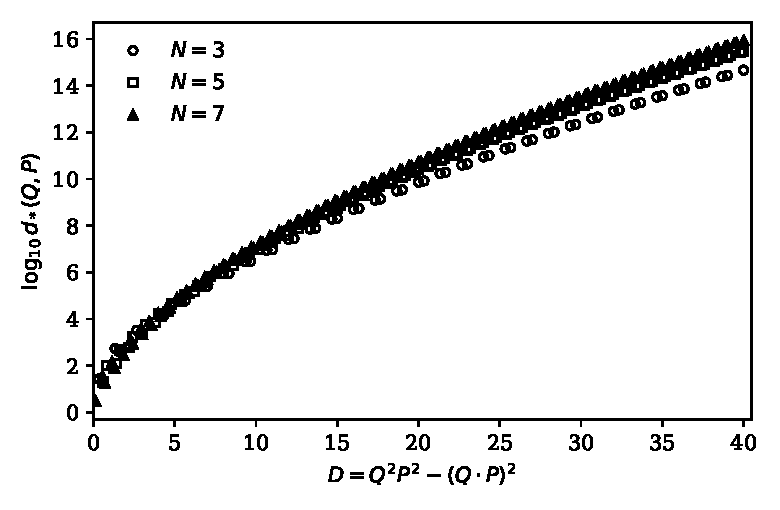
\includegraphics[width=0.7\textwidth]{fig_row1.pdf}
\caption{$\log_{10}d_*(Q,P)$ on the first row $Q^2=2/N$ for $0<D\le40$; circles $N=3$, squares $N=5$, filled triangles $N=7$. Every value is positive, as Theorem~\ref{thm:main} asserts.}
\label{fig:row1}
\end{figure}

\begin{figure}[t]
\centering
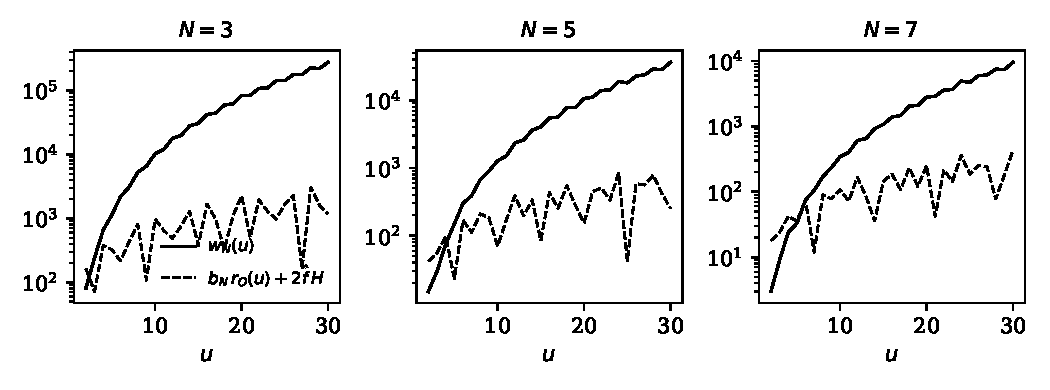
\includegraphics[width=\textwidth]{fig_bounds.pdf}
\caption{The positive term $w_N(u)$ (solid) against the bound $\frac{\hat f}6 r_\cO(u)+2\hat f H$ for the negative terms (dashed) in \eqref{eq:lb}, for $2\le u\le30$. The solid curve wins from $u=3,5,6$ on; the earlier values are covered by Table~\ref{tab:small}.}
\label{fig:bounds}
\end{figure}

%%==================================================================
\section{Toward All Charges}\label{sec:all}
%%==================================================================

For $N=2$ the proof of \cite{Bha26a} reduces every charge, by duality and the Fricke exchange, to one with $m\le n$ and $0\le\ell\le m$, writes $d_*$ as a Rademacher series over the cosets of $\Gamma_0(2)$, and shows that the terms attached to the leading family of walls resum to $|P(z)|^2$ with $P(z)=\prod_n(1-z^n)^{-8}(1-z^{2n})^{-8}$ on $|z|\le e^{-\pi}$, where $|P|^2\ge0.5389$. The same family for prime $N$ resums to $\prod_n|1-z^n|^{-2(k+2)}|1-z^{Nn}|^{-2(k+2)}$ on $|z|\le e^{-2\pi/N}$ \cite[Section~16]{Bha26a}. A grid evaluation on the boundary circle, where the minimum of the modulus is attained, gives the minima $0.2858$, $0.2202$ and $0.2024$ for $N=3,5,7$. These numbers are positive, so the method can work, but the error terms must be bounded below them rather than below $0.53$, and the Rademacher expansion for $\Gamma_0(N)$ requires the polar data of the finite parts at the cusp $0$ as well as at $\infty$. The first-row formula \eqref{eq:closed} gives these data exactly for $m=1$ and fixes the normalisation of the shadow, which is the natural starting point for that extension.

\subsection*{Data availability}
The Python programs that expand the product formula, compute the finite parts, verify Propositions~\ref{prop:num} and \ref{prop:theta} and the decompositions \eqref{eq:decomp}, check the small cases and the box of Section~\ref{sec:checks}, and draw the figures are available in the GitHub repository \url{https://github.com/anaxia-research/chl-positivity} (folder \texttt{code}), together with the source of this article.

\subsection*{Funding}
This research received no external funding.

\subsection*{Conflicts of interest}
The author declares no conflicts of interest.

\begin{thebibliography}{999}
\bibitem{Sen11} A. Sen, \emph{How do black holes predict the sign of the Fourier coefficients of Siegel modular forms?}, Gen. Relativ. Gravit. \textbf{43} (2011), 2171--2183. \href{https://doi.org/10.1007/s10714-011-1175-9}{doi:10.1007/s10714-011-1175-9}
\bibitem{Sen08} A. Sen, \emph{Black hole entropy function, attractors and precision counting of microstates}, Gen. Relativ. Gravit. \textbf{40} (2008), 2249--2431. \href{https://doi.org/10.1007/s10714-008-0626-4}{doi:10.1007/s10714-008-0626-4}
\bibitem{DVV97} R. Dijkgraaf, E. Verlinde, H. Verlinde, \emph{Counting dyons in $\mathcal N=4$ string theory}, Nucl. Phys. B \textbf{484} (1997), 543--561. \href{https://doi.org/10.1016/S0550-3213(96)00640-2}{doi:10.1016/S0550-3213(96)00640-2}
\bibitem{BM13} K. Bringmann, S. Murthy, \emph{On the positivity of black hole degeneracies in string theory}, Commun. Number Theory Phys. \textbf{7} (2013), 15--56. \href{https://doi.org/10.4310/CNTP.2013.v7.n1.a2}{doi:10.4310/CNTP.2013.v7.n1.a2}
\bibitem{Ros24} M. Rossell\'o, \emph{The immortal dyon index is positive}, preprint (2024). \href{https://arxiv.org/abs/2403.19630}{arXiv:2403.19630}
\bibitem{CHL95} S. Chaudhuri, G. Hockney, J. D. Lykken, \emph{Maximally supersymmetric string theories in $D<10$}, Phys. Rev. Lett. \textbf{75} (1995), 2264--2267. \href{https://doi.org/10.1103/PhysRevLett.75.2264}{doi:10.1103/PhysRevLett.75.2264}
\bibitem{JS06} D. P. Jatkar, A. Sen, \emph{Dyon spectrum in CHL models}, J. High Energy Phys. 2006, no.~4 (2006), 018. \href{https://doi.org/10.1088/1126-6708/2006/04/018}{doi:10.1088/1126-6708/2006/04/018}
\bibitem{DJS06} J. R. David, D. P. Jatkar, A. Sen, \emph{Product representation of dyon partition function in CHL models}, J. High Energy Phys. 2006, no.~6 (2006), 064. \href{https://doi.org/10.1088/1126-6708/2006/06/064}{doi:10.1088/1126-6708/2006/06/064}
\bibitem{BSS25} A. Bhand, A. Sen, R. K. Singh, \emph{Mock modularity in CHL models}, Res. Math. Sci. \textbf{12} (2025), 8. \href{https://doi.org/10.1007/s40687-024-00489-0}{doi:10.1007/s40687-024-00489-0}
\bibitem{Bha26a} D. Bhattacharjee, \emph{Every single-centred black hole index of the $\mathbb Z_2$ CHL model is positive}, Preprints (2026), version~2. \href{https://doi.org/10.20944/preprints202611.1118.v2}{doi:10.20944/preprints202611.1118.v2}
\bibitem{Bha26b} D. Bhattacharjee, \emph{Positive black hole indices in $\mathcal N=4$ and $\mathcal N=8$ string theory}, Preprints (2026), version~2. \href{https://doi.org/10.20944/preprints202611.1219.v2}{doi:10.20944/preprints202611.1219.v2}
\bibitem{EZ85} M. Eichler, D. Zagier, \emph{The Theory of Jacobi Forms}, Progress in Mathematics 55, Birkh\"auser, Boston, 1985. \href{https://doi.org/10.1007/978-1-4684-9162-3}{doi:10.1007/978-1-4684-9162-3}
\bibitem{Stu87} J. Sturm, \emph{On the congruence of modular forms}, in: Number Theory (New York, 1984--85), Lecture Notes in Math. 1240, Springer, Berlin, 1987, 275--280. \href{https://doi.org/10.1007/BFb0072985}{doi:10.1007/BFb0072985}
\bibitem{Zag75} D. Zagier, \emph{Nombres de classes et formes modulaires de poids $3/2$}, C. R. Acad. Sci. Paris S\'er. A \textbf{281} (1975), 883--886.
\bibitem{DMZ12} A. Dabholkar, S. Murthy, D. Zagier, \emph{Quantum black holes, wall crossing and mock modular forms}, preprint (2012). \href{https://arxiv.org/abs/1208.4074}{arXiv:1208.4074}
\bibitem{Voi21} J. Voight, \emph{Quaternion Algebras}, Graduate Texts in Mathematics 288, Springer, Cham, 2021. \href{https://doi.org/10.1007/978-3-030-56694-4}{doi:10.1007/978-3-030-56694-4}
\bibitem{Piz80} A. Pizer, \emph{An algorithm for computing modular forms on $\Gamma_0(N)$}, J. Algebra \textbf{64} (1980), 340--390. \href{https://doi.org/10.1016/0021-8693(80)90151-9}{doi:10.1016/0021-8693(80)90151-9}
\bibitem{Ono04} K. Ono, \emph{The Web of Modularity: Arithmetic of the Coefficients of Modular Forms and $q$-series}, CBMS Regional Conference Series in Mathematics 102, American Mathematical Society, Providence, 2004. \href{https://doi.org/10.1090/cbms/102}{doi:10.1090/cbms/102}
\bibitem{Del74} P. Deligne, \emph{La conjecture de Weil. I}, Publ. Math. IH\'ES \textbf{43} (1974), 273--307. \href{https://doi.org/10.1007/BF02684373}{doi:10.1007/BF02684373}
\end{thebibliography}

\end{document}
